\part{研发用户指南}

\section{通用陆面模式中的自定义数据类型}

\subsection{格点数据}
CoLM中使用的地表覆盖类型、土壤属性、叶面积指数、流域划分、湖泊深度和树高等细分辨率数据,以及大气驱动和历史输出等粗分辨率数据都是格点数据。

为了处理高分辨率数据和进行并行计算,CoLM对所有格点数据进行分块。分块方案为:通过设置Namelist文件中的\texttt{DEF\_nx\_blocks}和\texttt{DEF\_ny\_blocks}两个变量的值,将经向180\textdegree W至180\textdegree E等分为\texttt{DEF\_nx\_blocks}段,将纬向90\textdegree N至90\textdegree S等分为\texttt{DEF\_ny\_blocks}段。对区域模拟,同样指的是对全球进行分块。格点数据分块进行读取和使用,以双精度浮点型数据为例,在代码(share/MOD\_DataType.F90)中“格点数据”的自定义数据类型为
\begin{lstlisting}[language=fortran, basicstyle=\linespread{1.0}\footnotesize\ttfamily, commentstyle=\color{olive}, numbers=left, numberstyle=\tiny, xleftmargin=1.5em,xrightmargin=0em, aboveskip=1em]
   type :: pointer_real8_2d
      real(r8), allocatable :: val (:,:)
   CONTAINS
      final :: pointer_real8_2d_free_mem
   END type pointer_real8_2d

   type :: block_data_real8_2d
      type(pointer_real8_2d), allocatable :: blk (:,:)
   CONTAINS
      final :: block_data_real8_2d_free_mem
   END type block_data_real8_2d
\end{lstlisting}
此外,代码中还定义了整型格点数据以及三维、四维格点数据。

格点数据建立在固定的经纬度网格上,经纬度网格在CoLM中使用自定义数据结构“网格”进行描述。网格数据结构包含了每个数据块的经纬度信息、全局位置、数据大小以及其他辅助信息。以下代码展示了如何在网格grid上建立双精度浮点型格点数据gdata2d,
\begin{lstlisting}[language=fortran, basicstyle=\linespread{1.0}\footnotesize\ttfamily, commentstyle=\color{olive}, numbers=left, numberstyle=\tiny, xleftmargin=1.5em,xrightmargin=0em, aboveskip=1em]
    type(grid_type),           intent(in)  :: grid
    type(block_data_real8_2d), intent(out) :: gdata2d

    ! 在网格grid上建立双精度浮点型格点数据gdata2d
    CALL allocate_block_data (grid, gdata2d)
\end{lstlisting}
模式中对格点数据类型定义了析构函数,因此,使用格点数据的代码结束时,无需编写释放内存的代码。

从netCDF文件中读取格点数据可使用以下函数(其中filename和dataname分别为文件名和文件中的变量名),
\begin{lstlisting}[language=fortran, basicstyle=\linespread{1.0}\footnotesize\ttfamily, commentstyle=\color{olive}, numbers=left, numberstyle=\tiny, xleftmargin=1.5em,xrightmargin=0em, aboveskip=1em]
   CALL ncio_read_block (filename, dataname, grid, gdata2d)
\end{lstlisting}

若netCDF文件中的数据包含时间维度,可使用以下函数(其中itime为文件中时间维度的值),
\begin{lstlisting}[language=fortran, basicstyle=\linespread{1.0}\footnotesize\ttfamily, commentstyle=\color{olive}, numbers=left, numberstyle=\tiny, xleftmargin=1.5em,xrightmargin=0em, aboveskip=1em]
   CALL ncio_read_block_time (filename, dataname, grid, itime, gdata2d)
\end{lstlisting}

以上函数allocate\_block\_data, ncio\_read\_block, ncio\_read\_block\_time对整型、浮点型以及二维、三维数据做了重载,因此,使用时函数名中未加数据类型及维数。

对格点数据的定位需要同时使用分块信息和网格信息,以下代码展示了如何对格点数据进行操作,
\begin{lstlisting}[language=fortran, basicstyle=\linespread{1.0}\footnotesize\ttfamily, commentstyle=\color{olive}, numbers=left, numberstyle=\tiny, xleftmargin=1.5em,xrightmargin=0em, aboveskip=1em]
    IF (p_is_io) THEN
        DO iblkme = 1, gblock%nblkme
            ib = gblock%xblkme(iblkme)
            jb = gblock%yblkme(iblkme)

            DO j = 1, grid%ycnt(jb)
                DO i = 1, grid%xcnt(ib)
                    ! 对gdata2d%blk(ib,jb)%val(i,j)进行操作
                ENDDO
            ENDDO
        ENDDO
    ENDIF
\end{lstlisting}
这段代码中,首先判断本进程是否为IO进程(格点数据仅位于读写进程的内存中,见第\ref{ch_parallel}节)。若是,则从gblock变量中循环获取分配给本进程的数据块的位置(代码中的ib和jb)。对分配给本进程的每个数据块,可进一步通过循环(代码中的j和i),对每个网格点上的数据进行操作。

\subsection{向量数据}

CoLM中的斑块(patch)、流域单元、非结构网格单元、水文响应单元、植被功能类型单元和植物群落单元等都具有不规则的形状,这些不规则形状单元在模式中使用细分辨率格点的集合进行表示。例如,使用0.5\textdegree 度经纬度网格单元进行陆面过程模拟时,在单元内部使用500米分辨率的地表覆盖类型数据建立次网格斑块单元,此时,一个斑块单元表示在一个0.5\textdegree 网格内部具有相同地表覆盖类型的500米细分辨率格点的集合。又如,使用流域单元进行陆面过程模拟时,根据90米高分辨率的水文学数据对模拟区域进行流域单元的划分,一个流域单元在模式中表示为90米细分辨率的格点的集合。

定义在不规则形状单元上的变量在模式中使用“向量”数据结构,为一维、二维或者三维数组,数组的最后一个维度的长度等于不规则单元的数量。例如定义在斑块上的叶面积指数
\begin{lstlisting}[language=fortran, basicstyle=\linespread{1.0}\footnotesize\ttfamily, commentstyle=\color{olive}, numbers=left, numberstyle=\tiny, xleftmargin=1.5em,xrightmargin=0em, aboveskip=1em]
    IF (p_is_worker) THEN
       allocate (lai (numpatch))
    ENDIF
\end{lstlisting}
这段代码中,首先判断本进程是否为worker进程(向量数据仅位于工作进程的内存中,见第\ref{ch_parallel}节)。若是,则定义一个一维数组存储叶面积指数的值,其长度等于分配到本进程的斑块的数量(numpatch)。

\subsection{格点数据和向量数据之间的映射}

陆面模式的输入数据(地表数据、大气驱动数据等)多为格点数据,而模式的基本单元为斑块等不规则单元,因此,需将格点数据映射到网格数据。CoLM中主要使用两种将格点数据映射到向量数据的方法,一种是面积加权平均,另一种是双线性插值。

以下代码定义和构建了由格点数据向斑块单元的面积加权平均映射,
\begin{lstlisting}[language=fortran, basicstyle=\linespread{1.0}\footnotesize\ttfamily, commentstyle=\color{olive}, numbers=left, numberstyle=\tiny, xleftmargin=1.5em,xrightmargin=0em, aboveskip=1em]
    type (grid_type) :: gforc
    type (pixelset_type) :: landpatch
    type (spatial_mapping_type) :: mg2p_forc

    ! 构建由定义在网格gforc上的格点数据向斑块单元的面积加权平均映射
    CALL mg2p_forc%build_arealweighted (gforc, landpatch)
\end{lstlisting}
具体实现时,面积加权平均方法先将格点数据映射到不规则单元内的细网格上,再对细网格进行加权平均,其可保证在映射的过程中变量是守恒的。上述映射只需在初始化时构建一次,调用以下函数进行使用
\begin{lstlisting}[language=fortran, basicstyle=\linespread{1.0}\footnotesize\ttfamily, commentstyle=\color{olive}, numbers=left, numberstyle=\tiny, xleftmargin=1.5em,xrightmargin=0em, aboveskip=1em]
    CALL mg2p_forc%grid2pset (forc_xy_t, forc_t)
\end{lstlisting}
其中,forc\_xy\_t为格点数据,forc\_t为向量数据。

以下代码定义和构建了由格点数据向斑块单元的双线性插值映射,
\begin{lstlisting}[language=fortran, basicstyle=\linespread{1.0}\footnotesize\ttfamily, commentstyle=\color{olive}, numbers=left, numberstyle=\tiny, xleftmargin=1.5em,xrightmargin=0em, aboveskip=1em]
    type (grid_type) :: gforc
    type (pixelset_type) :: landpatch
    type (spatial_mapping_type) :: mg2p_forc

    ! 构建由定义在网格gforc上的格点数据向斑块单元的双线性插值映射
    CALL mg2p_forc%build_bilinear (gforc, landpatch)
\end{lstlisting}
具体实现时,双线性映射方法将格点数据视为定义在经纬度网格点的中心位置,向量数据视为定义在不规则单元的重心位置,由包围不规则单元重心点的四个网格中心点向不规则单元进行插值。单独的双线性映射方法不能保证变量的守恒性,但与面积加权平均方法相比,使得插值后的变量在空间上较为平滑。上述映射同样只需在初始化时构建一次,调用以下函数进行使用
\begin{lstlisting}[language=fortran, basicstyle=\linespread{1.0}\footnotesize\ttfamily, commentstyle=\color{olive}, numbers=left, numberstyle=\tiny, xleftmargin=1.5em,xrightmargin=0em, aboveskip=1em]
    CALL mg2p_forc%grid2pset (forc_xy_t, forc_t)
\end{lstlisting}
其中,forc\_xy\_t为格点数据,forc\_t为向量数据。

模式结果通常以格点数据的方式输出,以增强可视化和结果分析的便利性,因此,需在输出时将定义在基本模拟单元上的向量数据映射到格点数据。向量数据向格点数据映射的构建与上述格点数据向向量数据映射的构建是相同的,使用时,以下函数
\begin{lstlisting}[language=fortran, basicstyle=\linespread{1.0}\footnotesize\ttfamily, commentstyle=\color{olive}, numbers=left, numberstyle=\tiny, xleftmargin=1.5em,xrightmargin=0em, aboveskip=1em]
    CALL mp2g_hist%pset2grid (hist_t, hist_xy_t, spv = filledvalue, msk = filter)
\end{lstlisting}
执行向量数据hist\_t向格点数据hist\_xy\_t的映射,其中spv和msk为两个可选参数。浮点数spv表示计算过程中不予考虑的填充值。msk为逻辑型向量数据,其第i个元素值为\texttt{TRUE}时表示此不规则单元参与映射,值为\texttt{FALSE}时表示不参与映射。例如,在输出湖泊温度时,可使用msk变量,将所有湖泊单元表示出来进行映射和输出。值得注意的是,当从向量数据向格点数据进行映射时,执行函数mp2g\_hist\%pset2grid得到的结果hist\_xy\_t表示格点内变量的总量,若要计算变量的均值,可先执行
\begin{lstlisting}[language=fortran, basicstyle=\linespread{1.0}\footnotesize\ttfamily, commentstyle=\color{olive}, numbers=left, numberstyle=\tiny, xleftmargin=1.5em,xrightmargin=0em, aboveskip=1em]
    CALL mp2g_hist%get_sumarea (sumarea, filter)
\end{lstlisting}
得到格点内参与映射的不规则单元的总面积sumarea,然后在每个格点内用变量的总量除以总面积得到均值。


\section{并行计算构架}\label{ch_parallel}

CoLM 2024版使用MPI(Massage Passing Interface)函数库实现在多核小型机、服务器以及超级计算机上的并行计算。

当使用多个进程运行模式时,所有进程被分为四类(见图~\ref{fig:fig_parallelization}),分别为主进程、读写进程、工作进程和回写进程。主进程(master)处理全局的输入输出和在运行过程中打印信息。读写进程(IO)进行数据的分发、收集和读写。工作进程(worker)执行模式过程。回写进程为可选项,专门用于历史文件的写出。一个工作组由一个读写进程和多个工作进程组成。

\begin{figure}[htpb]
    \centering
    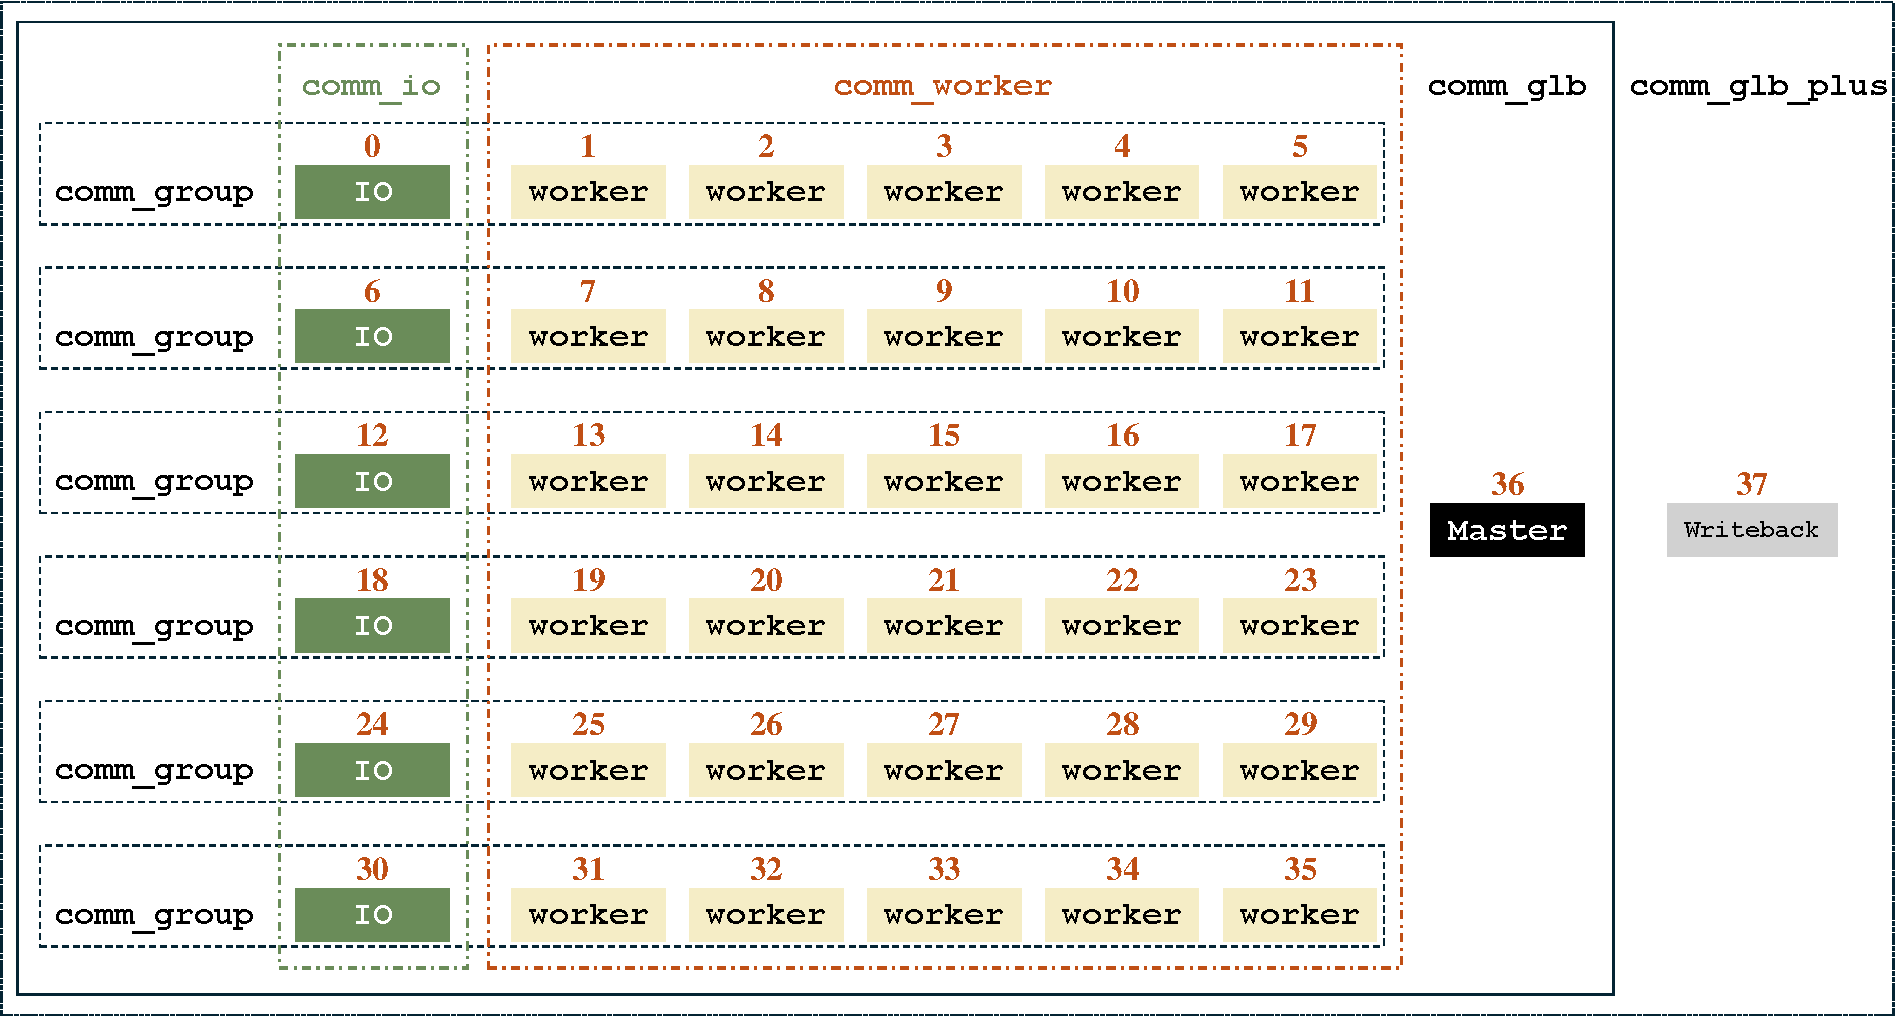
\includegraphics[width=\textwidth]{figures/并行计算图.pdf}
    \caption{CoLM 2024版并行计算构架示意图。其中所有进程被分为四类,分别为主进程、读写进程、工作进程和回写进程,数字标号0\textasciitilde 37为进程的全局编号。comm\_group为一个读写进程和多个工作进程组成的工作组通讯域,comm\_io为所有读写进程组成的通讯域,comm\_worker为所有工作进程组成的通讯域,comm\_glb为主进程、读写进程和工作进程组成的通讯域,comm\_glb\_plus为所有进程的通讯域。}
    \label{fig:fig_parallelization}
\end{figure}

并行运行模式时,模式以加权轮询的方式将数据块分配到工作组(见图~\ref{fig:fig_block}),每个工作组主要负责其分配到的数据块上的读写和模式计算。在工作组内,工作任务的分配以陆表单元(Element)为基本单位,每个陆表单元内部进一步划分的水文响应单元(HRU)、次网格单元(patch)、植被功能类型单元(PFT)以及植被群落单元(PC)等都分配到同一个进程上。工作组内任务的分配方法为将每个数据块上的陆表单元均匀分配,例如,某数据块有150个陆表单元,负责其计算的工作组有4个工作进程,将陆表单元按编号排序后,第1到4个工作进程分别进行第1到38、第39到76,第77到113,第114到150个陆表单元上的模拟。

\begin{figure}[htpb]
    \centering
    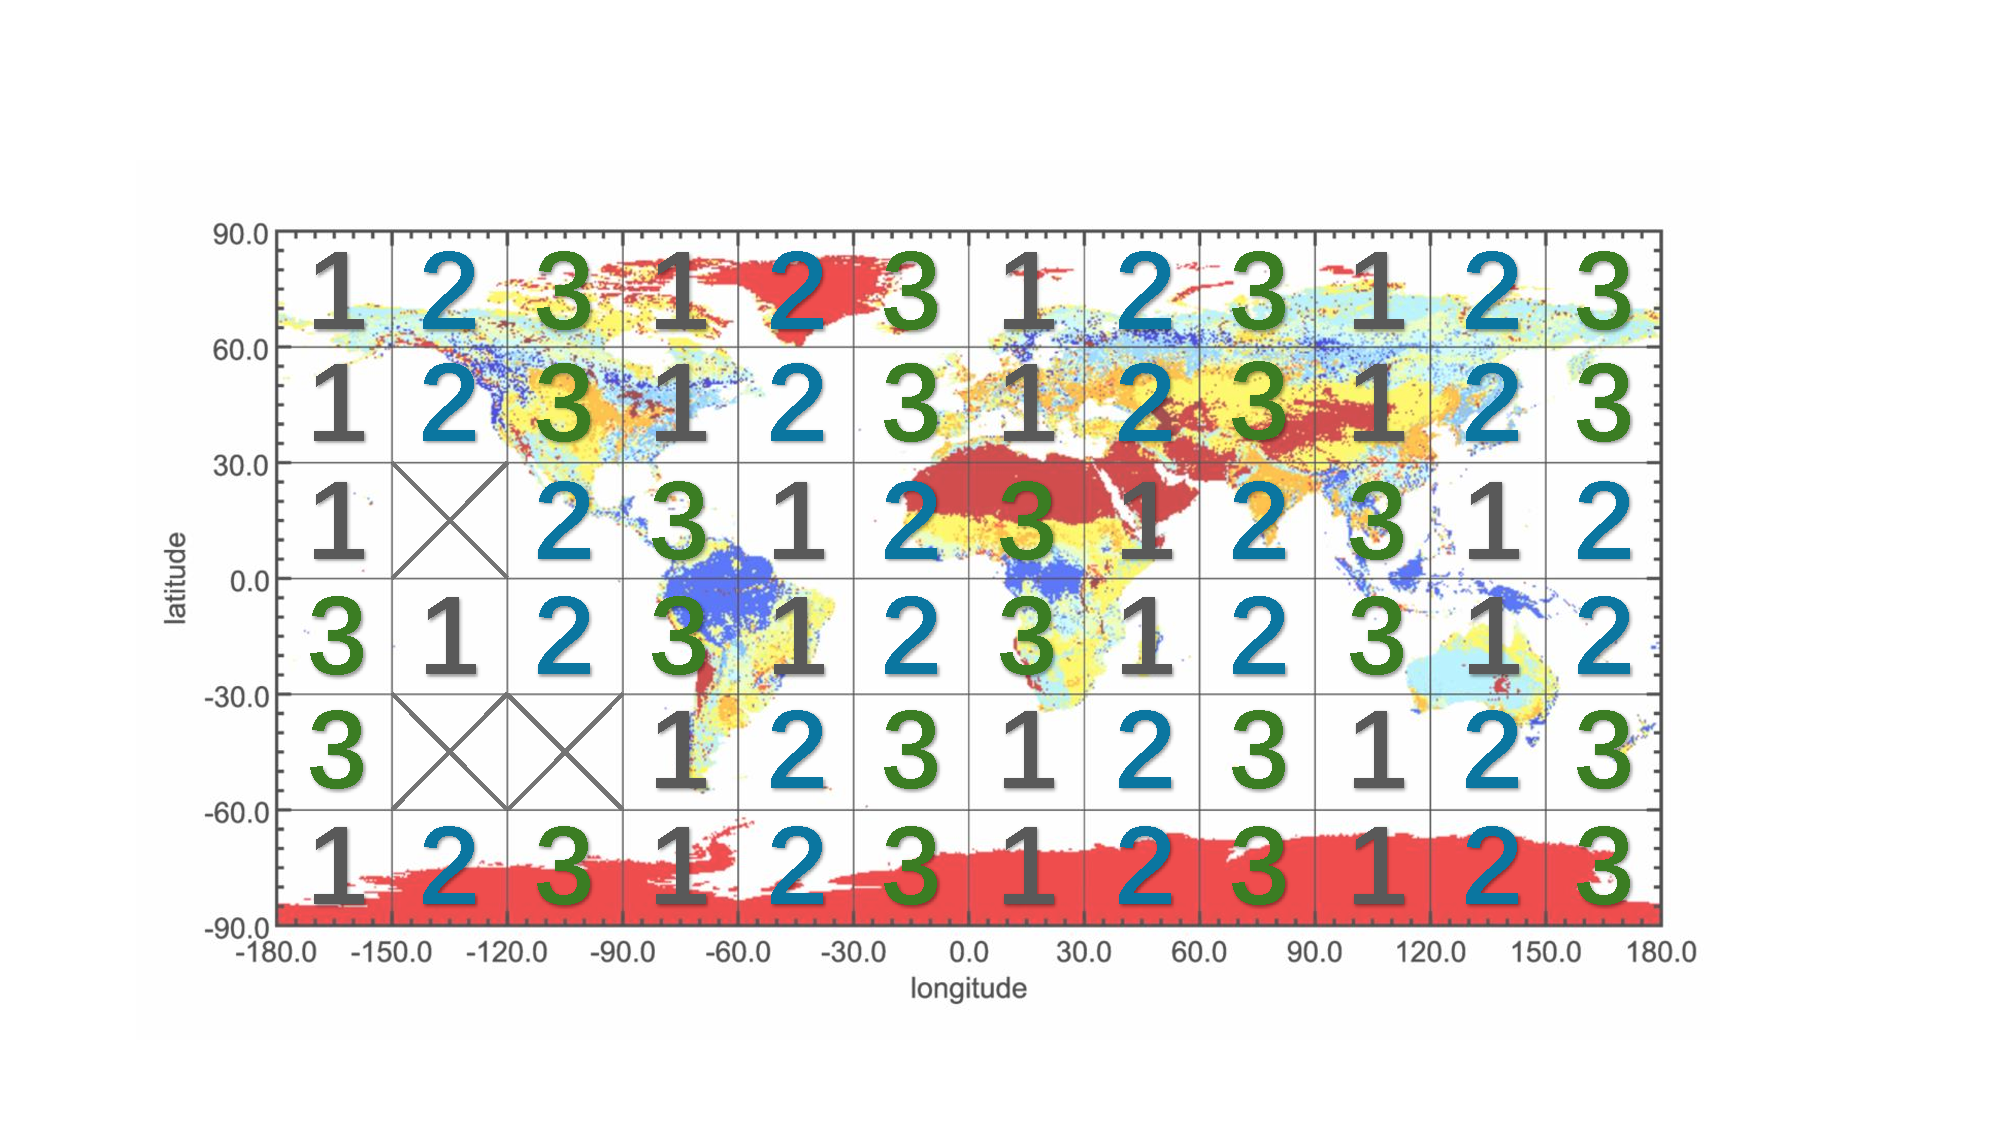
\includegraphics[width=\textwidth]{figures/数据分块示意图.pdf}
    \caption{CoLM 2024版数据分块及并行任务分配示意图。本例中将全球分为30\textdegree$\times$ 30\textdegree 的数据块。当使用3个工作组运行模式时,数据分块以轮询的方式分配到工作组,图中的数字1,2,3表示负责该数据块的工作组的编号。}
    \label{fig:fig_block}
\end{figure}

格点数据主要储存在读写进程(IO)的内存中,其读写有多种方式,可适应不同的计算环境。读入格点数据时,每个读写进程直接从外部文件中读入其负责的数据块上的数据。向外部文件写入格点数据有三种方式。第一种方式,当\texttt{DEF\_HIST\_mode}为'block'时,读写进程将每个数据块的内容写入单独的文件,这种方式通常具有最高的写文件速度,但分析结果时需要后处理程序拼接数据。第二种方式,当\texttt{DEF\_HIST\_mode}为'one'且\texttt{DEF\_HIST\_WriteBack}为\texttt{FALSE}时,由主进程在运行过程中从读写进程收集所有数据块的数据,进行拼接后将完整数据写出,这种方式不需要进行后期数据处理,但因收集数据时使用了阻塞通讯,在数据量较大时效率低、耗时长。第三种方式,当\texttt{DEF\_HIST\_mode}为'one'且\texttt{DEF\_HIST\_WriteBack}为\texttt{TRUE}时,模式将全局编号最大的进程独立出来作为回写进程,回写进程在运行过程中从读写进程收集所有数据块的数据,进行拼接后将完整数据写出,与第二种方式不同的是,读写进程向回写进程发送数据块上的数据时,使用的是非阻塞通讯,可不等待数据接收完成就继续向下运行。

向量数据主要储存在工作进程(worker)的内存中,其读写需通过读写进程(IO)。从外部文件读取向量数据时,读写进程首先读入其负责的数据块上的向量数据的子集,再分发给其工作组中的工作进程,分发过程通过进程之间的通讯实现。当向外部文件写入向量数据时,读写进程首先通过进程之间的通讯从其工作组中的工作进程收集数据,再按数据块将数据写入独立的文件。

因格点数据和向量数据分别位于读写进程和工作进程的内存中,格点数据和向量数据之间的映射均需通过进程之间的通讯实现。离线模拟时,大气驱动数据通常为格点数据,由读写进程读入后,按需发送至工作进程,再映射到向量数据。以经纬度网格进行历史数据输出时,需从工作进程发送以向量数据为形式的模拟结果至读写进程,再由读写进程累加到格点上。这些数据收发和累加映射的函数已封装在模块MOD\_SpatialMapping中,一般不需要开发者自己改写代码。

% \section{网格的定义}
